%!TEX root = ../Dimensionieren I.tex

\label{chap:ermuedungsfestigkeit}
Bemerkung: Der Index \textbf{a} kennzeichnet die \textbf{vorliegende Spannung} \textbf{A} die \textbf{ertragbare Spannung}.

\section{Vorgehen} % (fold)
	\begin{enumerate}
		\item Kritische Querschnitte bestimmen.
		\item Beanspruchung im gewählten Querschnitt:
			\begin{enumerate}
				\item Normalspannung $\sigma_{\text{zd}}$.
				\item Biegespannung $\sigma_{\text{b}}$.
				\item Torsionsspannung $\tau_{\text{t}}$.
			\end{enumerate}
		\item Gestaltfestigkeit:
			\begin{enumerate}
				\item Wechselfestigkeit (meist tabelliert) \\
				$\Rightarrow \sigma_\text{zdW}, \sigma_\text{bW}, \tau_\text{tW}$.
				\item Technologischer Grösseneinflussfaktor (materialabhängig) $\Rightarrow K_1$.
				\item Einfluss einer Oberflächenverfestigung $\Rightarrow K_{\text{V}}$.
				\item Kerbwirkungszahl $\Rightarrow \beta_\sigma, \beta_\tau$.
				\item Geometrischer Grösseneinflussfaktor $\Rightarrow K_2$.
				\item Einfluss der Oberflächenrauheit $\Rightarrow K_{\text{F}}$.
			\end{enumerate}
		\item Einflussfaktor der Mittelspannung (meist 0): $\Rightarrow \Psi_{\text{K}}$.
		\item Spannungsamplituden: $\Rightarrow \sigma_{\text{zda}}, \sigma_{\text{ba}}, \tau_{\text{ta}}$.
		\item Vergleichsausschlagsspannung $\Rightarrow \sigma_{\text{Va}}$.
		\item Gestaltfestigkeit $\Rightarrow \sigma_{\text{VADK}}$.
		\item Sicherheit: $\Rightarrow S_{\text{B}}$.
	\end{enumerate}
% section: Vorgehen (end)
\section{Gestaltfestigkeit} % (fold)
	Zug / Druck:
	\begin{equation*}
		\sigma_{\text{zdWK}} = \frac{\sigma_{\text{zdW}}(d_{\text{B}}) \cdot K_1(d) \cdot K_{\text{V}}}{\left( \frac{\beta_{\sigma\text{, Zug}}}{K_2(d)} + \frac{1}{K_{\text{F,}\sigma}} - 1\right)}
	\end{equation*}
	Biegung:
	\begin{equation*}
		\sigma_{\text{bWK}} = \frac{\sigma_{\text{bW}}(d_{\text{B}}) \cdot K_1(d) \cdot K_{\text{V}}}{\left( \frac{\beta_{\sigma\text{, Bieg}}}{K_2(d)} + \frac{1}{K_{\text{F,}\sigma}} - 1\right)}
	\end{equation*}
	Torsion:
	\begin{equation*}
		\tau_{\text{zdWK}} = \frac{\tau_{\text{tW}}(d_{\text{B}}) \cdot K_1(d) \cdot K_{\text{V}}}{\left( \frac{\beta_{\tau}}{K_2(d)} + \frac{1}{K_{\text{F,}\tau}} - 1\right)}
	\end{equation*}
	
	\subsection{Wechselfestigkeit} % (fold)
		Näherungen für Stahl:
		\begin{equation*}
			\sigma_{\text{zdW}}(d_{\text{B}}) \approx 0.4 \cdot \sigma_{\text{B}}
		\end{equation*}
		\begin{equation*}
			\sigma_{\text{bW}}(d_{\text{B}}) \approx 0.5 \cdot \sigma_{\text{B}}
		\end{equation*}
		\begin{equation*}
			\tau_{\text{tW}}(d_{\text{B}}) \approx 0.3 \cdot \sigma_{\text{B}}
		\end{equation*}
		Tabellenwerte:
		\begin{enumerate}
			\item Allgemeine Baustähle $\rightarrow$ siehe \emph{\ref{baustaehle}}.
			\item Einsatzstähle $\rightarrow$ siehe \emph{\ref{einsatzstaehle}}.
			\item Vergütungsstähle $\rightarrow$ siehe \emph{\ref{verguetungsstaehle}}.
			\item Nitrierstähle $\rightarrow$ siehe \emph{\ref{nitrierstaehle}}.
		\end{enumerate}
	% subsection: Wechselfestigkeit (end)
	\subsection{Einfluss der Wärmebehandlung -- Technologischer Grösseneinflussfaktor} % (fold)
		Der technologische Grösseneinflussfaktor korrigiert Festigkeitswerte, die für einen bestimmten Bezugsdurchmesser gelten:
		\begin{equation*}
			\sigma_{\text{G}}(d) = K_1(d)\cdot \sigma_{\text{G}}(d_{\text{B}}), \qquad
			\sigma_{\text{G}} = \conditional{
				\sigma_{\text{S}} & \text{für Fliessgrenze} \\
				\sigma_{\text{B}} & \text{für Zugfestigkeit}
			}
		\end{equation*}
		
		\begin{center}
			\begin{tabular}{l|lr@{$\:=\:$}l}
				\toprule
				\multicolumn{4}{l}{\textbf{Allgemeine Baustähle}} \\
				\midrule
				\multirow{3}{*}{
				\begin{sideways}
					$d_\text{B} = 16$
				\end{sideways}
				} & $\sigma_\text{S}(d\leq 32)$ & $K_1(d)$ & $1$ \\
				 & $\sigma_\text{S}(32 < d < 300)$ & $K_1(d)$ & $1-0.26 \log \parens{\nicefrac{d}{2d_\text{B}}}$ \\
				 & $\sigma_\text{S}(300 \leq d \leq 500)$ & $K_1(d)$ & $0.75$ \\
				\midrule
				\multirow{3}{*}{
				\begin{sideways}
					$d_\text{B} = 100$
				\end{sideways}
				} & $\sigma_\text{B}(d \leq 100)$ & $K_1(d)$ & $1$ \\
				& $\sigma_\text{B}(100 < d < 300)$ & $K_1(d)$ & $1-0.23\log\parens{\nicefrac{d}{d_\text{B}}}$ \\
				& $\sigma_\text{B}(300 \leq d \leq 500)$ & $K_1(d)$ & $0.89$ \\
				\midrule \midrule
				\multicolumn{4}{l}{\textbf{Einsatzstähle} (ohne Cr-Ni-Mo-Einsatzstähle)} \\
				\midrule
				\multirow{3}{*}{
				\begin{sideways}
					$d_\text{B} = 11$
				\end{sideways}
				} & $\sigma_\text{S,B}(d\leq 11)$ & $K_1(d)$ & $1$ \\
				& $\sigma_\text{S,B}(11 < d < 300)$ & $K_1(d)$ & $1-0.41\log\parens{\nicefrac{d}{d_\text{B}}}$ \\
				& $\sigma_\text{S,B}(300 \leq d \leq 500)$ & $K_1(d)$ & $0.41$ \\
				\midrule \midrule
				\multicolumn{4}{l}{\textbf{Vergütungsstähle} (inkl.~Cr-Ni-Mo-Einsatzstähle)} \\
				\midrule
				\multirow{3}{*}{
				\begin{sideways}
					$d_\text{B} = 16$
				\end{sideways}
				} & $\sigma_\text{S,B}(d\leq 16)$ & $K_1(d)$ & $1$ \\
				& $\sigma_\text{S,B}(16 < d < 300)$ & $K_1(d)$ & $1-0.26\log\parens{\nicefrac{d}{d_\text{B}}}$ \\
				& $\sigma_\text{S,B}(300 \leq d \leq 500)$ & $K_1(d)$ & $0.67$ \\
				\midrule \midrule
				\multicolumn{4}{l}{\textbf{Nitrierstähle}} \\
				\midrule
				\multirow{3}{*}{
				\begin{sideways}
					$d_\text{B} = 100$
				\end{sideways}
				} & $\sigma_\text{S,B}(d\leq 100)$ & $K_1(d)$ & $1$ \\
				& $\sigma_\text{S,B}(100 < d < 300)$ & $K_1(d)$ & $1-0.23\log\parens{\nicefrac{d}{d_\text{B}}}$ \\
				& $\sigma_\text{S,B}(300 \leq d \leq 500)$ & $K_1(d)$ & $0.89$ \\
				\bottomrule
			\end{tabular}
		\end{center}
	% subsection: Technologischer Grösseneinflussfaktor (end)
	\subsection{Einfluss der Oberflächenverfestigung} % (fold)
		\begin{center}
			\begin{tabular}{llr@{.}l}
				\toprule
				\textbf{Verfahren} & \textbf{Durchmesser} & \multicolumn{2}{l}{$\boldsymbol{K_{\textbf{V}}}$ \textbf{(min)}} \\
				\midrule
				Nitrieren & $8 < d < 25$ & 1&15 \\
				& $25 < d < 40$ & 1&1 \\
				\midrule
				Einsatzhärten & $8 < d < 25$ & 1&2 \\
				 & $25 < d < 40$ & 1&1 \\
				\midrule
				Karbonnitrieren & 10 & 1&8 \\
				\midrule
				Rollen & $7<d<25$ & 1&2 \\
				 & $25<d<40$ & 1&1 \\
				\midrule
				Kugelstrahlen & $7<d<40$ & 1&1\\
				\bottomrule
			\end{tabular}
		\end{center}
		Für $d > 40$ wird $K_\text{V} = 1$ eingesetzt. Falls keine Bearbeitung der Oberfläche vorliegt, ist $K_V = 1$.
	% subsection: Einfluss der Oberflächenverfestigung (end)
	\subsection{Kerbwirkungszahl} % (fold)
		Dauerfestigkeit der gekerbten Probe:
		\begin{equation*}
			\sigma_{\text{ADK}} = \frac{\sigma_{\text{AD}}}{\beta_{\sigma,\tau}}
		\end{equation*}
		
		\paragraph{Passfedern}
		Empfehlungen:
		\begin{equation*}
			\frac{R}{d-d_1} = 2, \qquad \frac{d}{d_1}=1.1
		\end{equation*}
		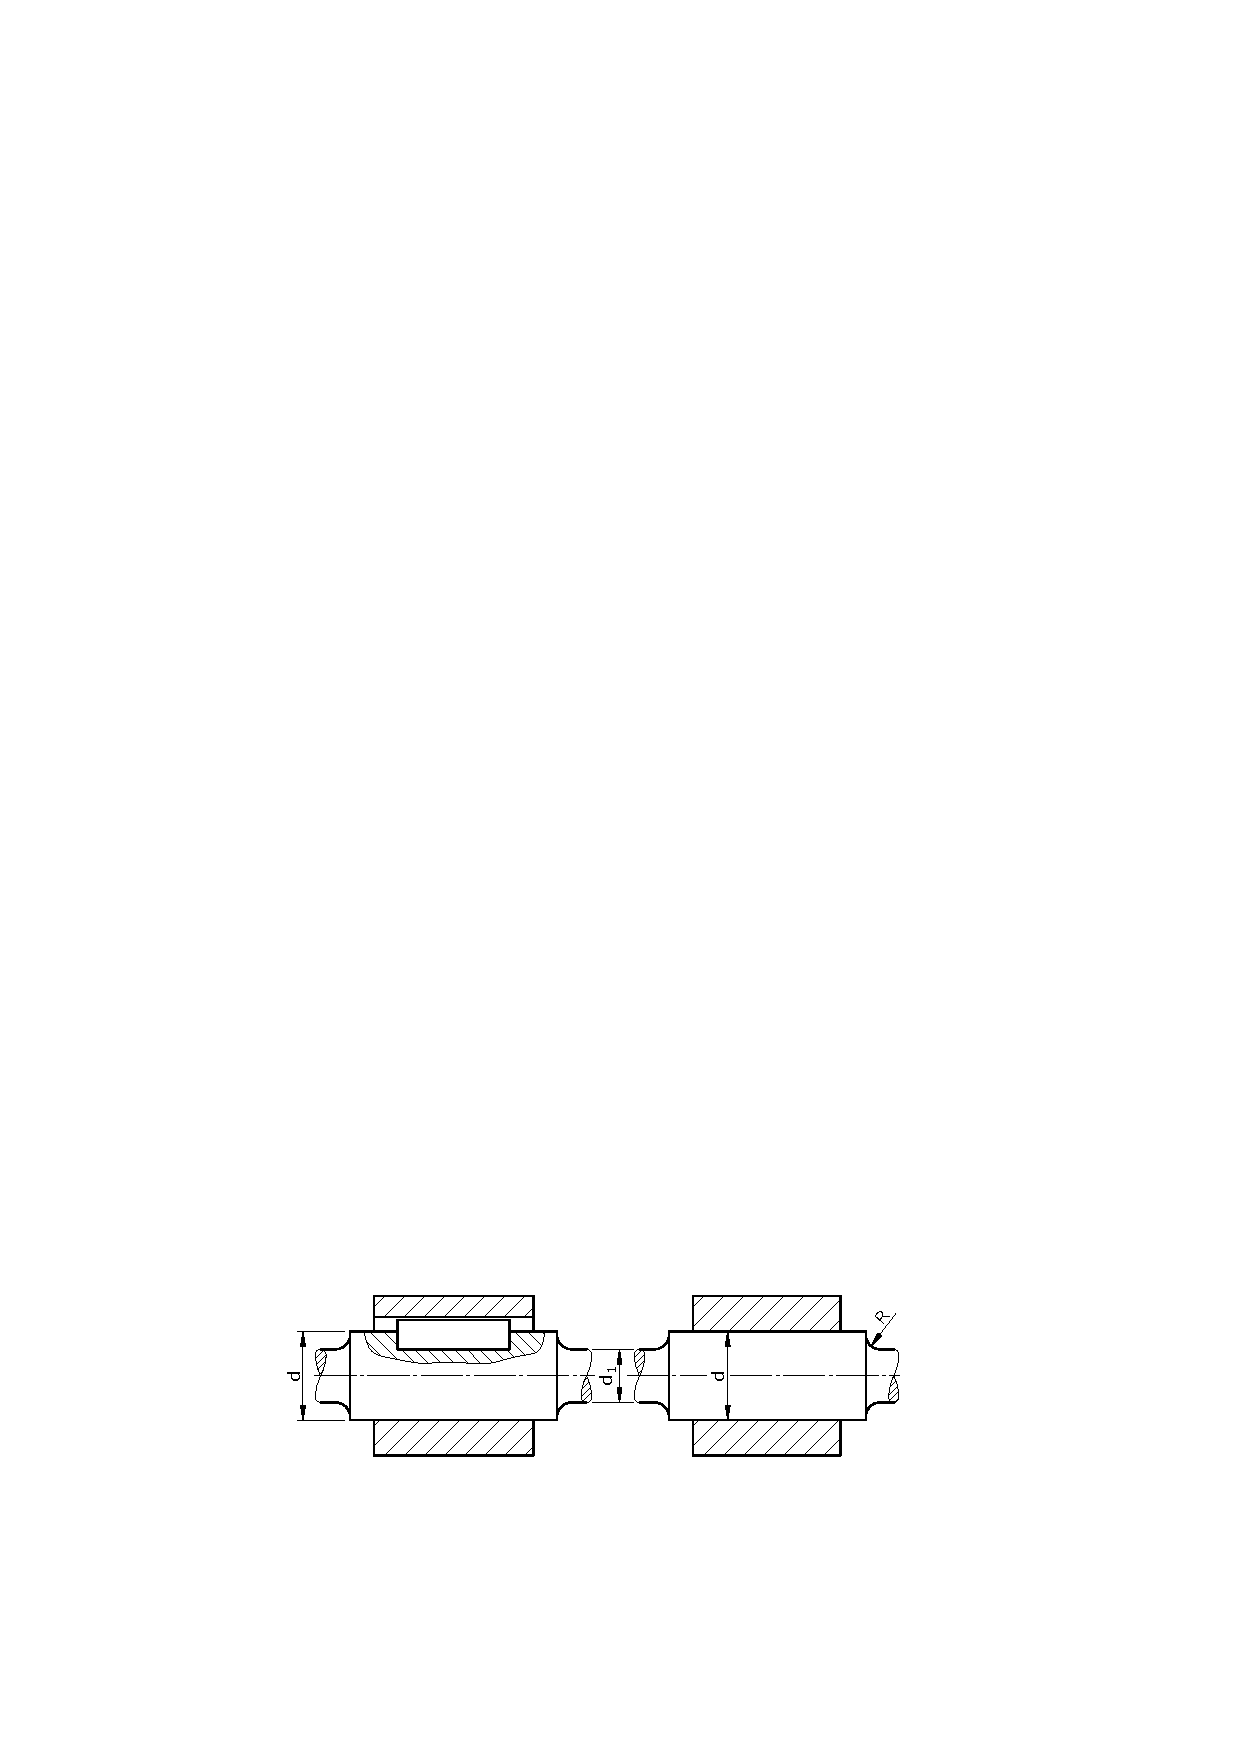
\includegraphics[width=\columnwidth]{graphics/passfedern}
		
		\paragraph{Umlaufende Spitzkerbe}~\\
		\begin{equation*}
			d_{\text{B}}=15, \qquad 0.05<\frac{D-d}{d}<0.2
		\end{equation*}
		\begin{tabular}{rr@{$\:=\:$}l}
			Zug/Druck: & $\beta_\sigma (d_\text B)$ & $\displaystyle 0.109 \frac{\sigma_\text{B}(d_\text B)}{100} + 1.074$ \\[2ex]
			Biegung: & $\beta_\sigma (d_\text B)$ & $\displaystyle 0.0923 \frac{\sigma_\text{B}(d_\text B)}{100}+0.985$ \\[2ex]
			Torsion: & $\beta_\tau (d_\text B)$ & $0.8 \: \beta_{\sigma\text{,Biegung}}$
		\end{tabular}
		
		\begin{center}
			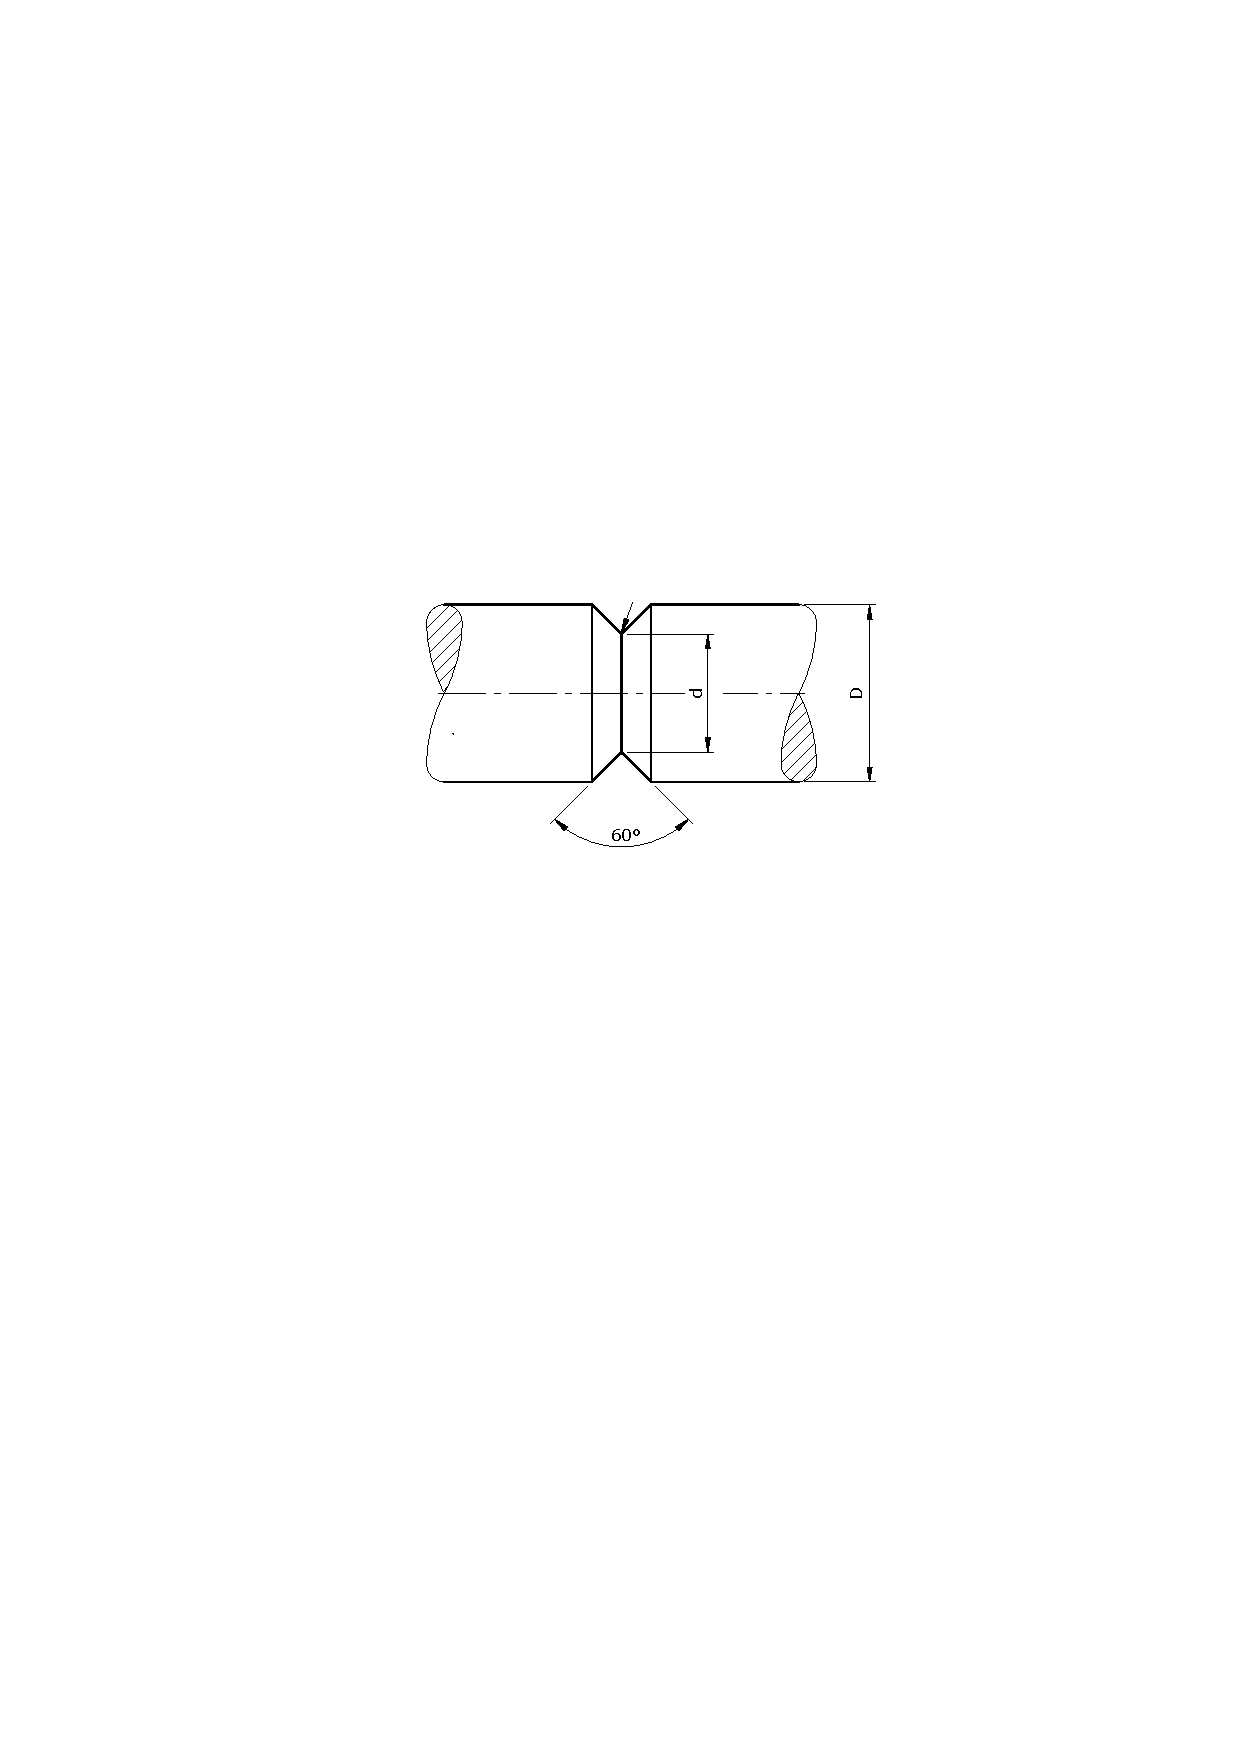
\includegraphics[]{graphics/spitzkerbe}
		\end{center}
		
		\paragraph{Rechtecknut}
		\begin{equation*}
			d_{\text{B}}= 15
		\end{equation*}
		\begin{center}
			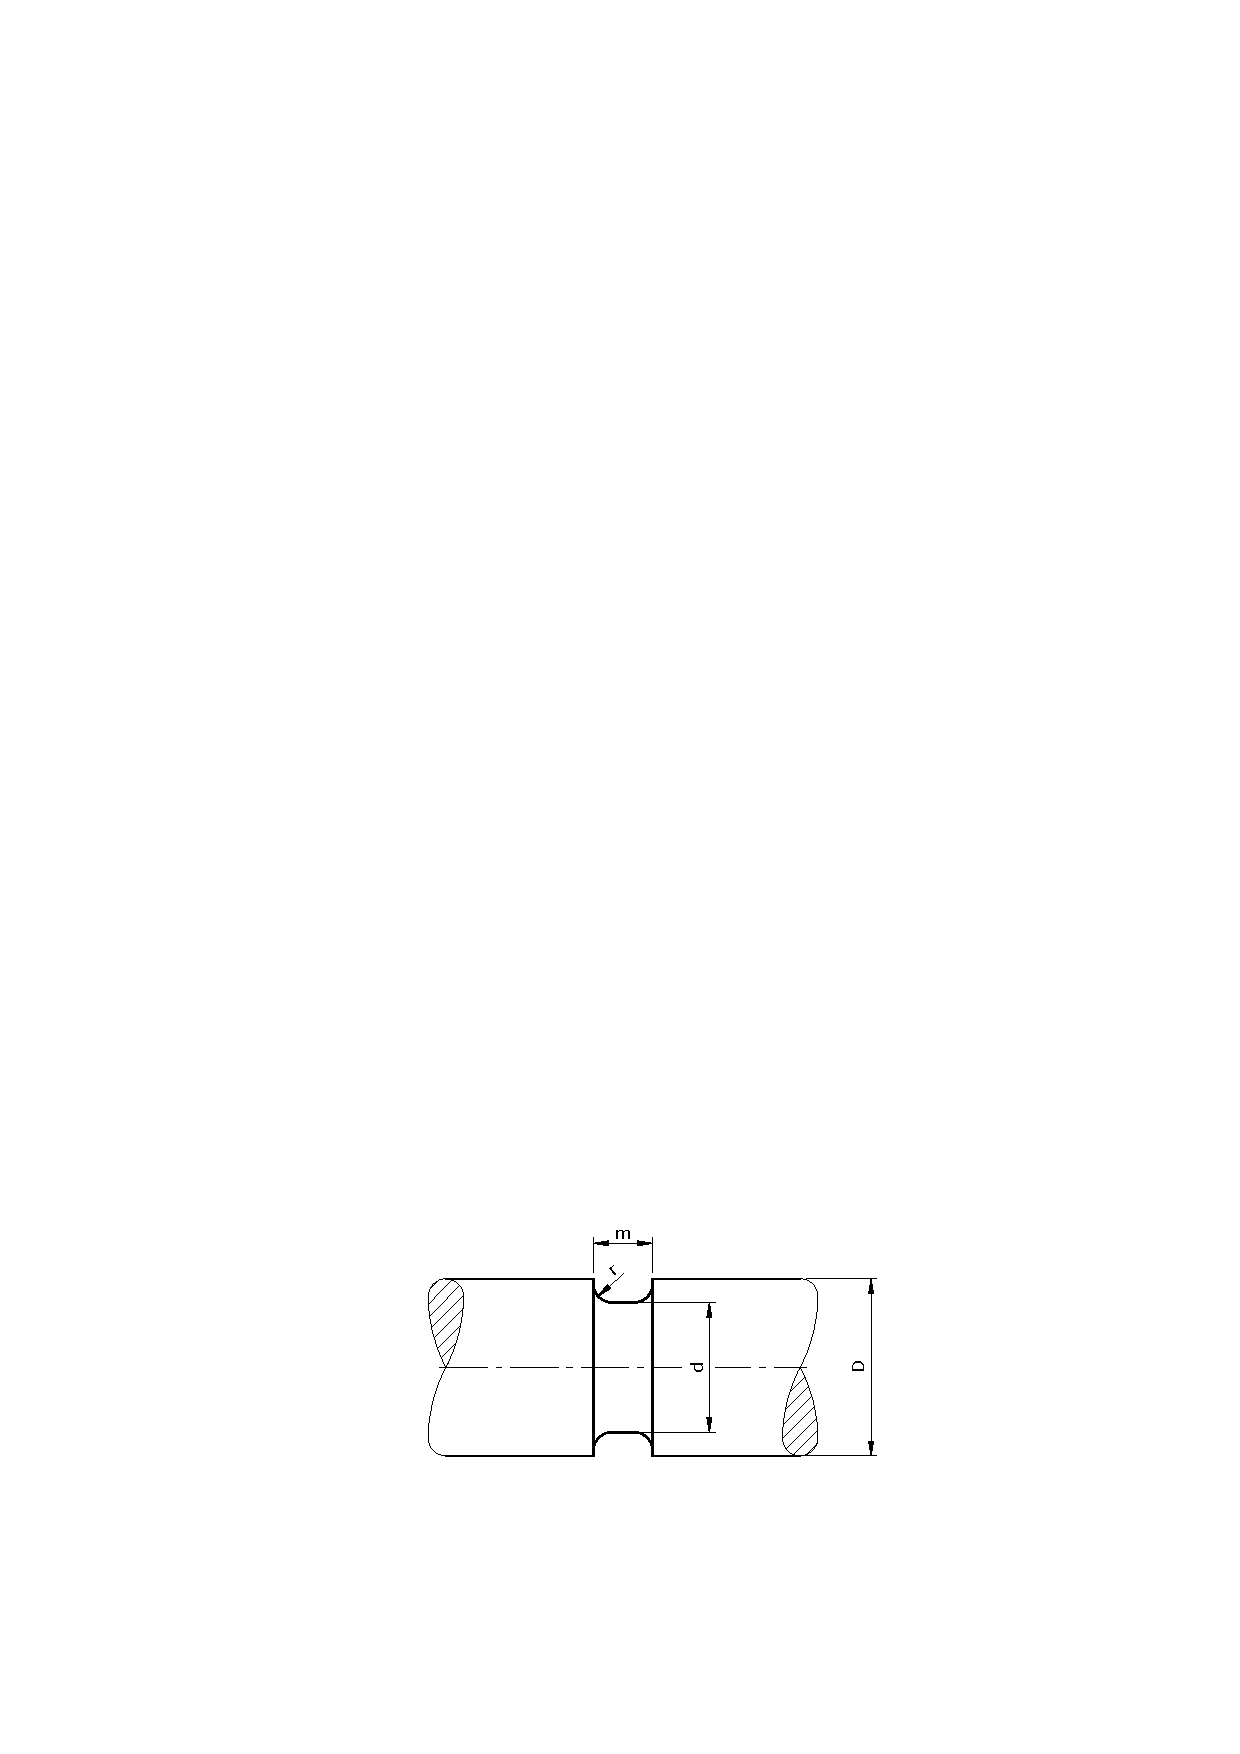
\includegraphics[]{graphics/rechtecknut}
		\end{center}
		
		\begin{tabular}{rr@{$\:=\:$}l}
			Zug/Druck: & $\beta_\sigma (d_\text B)$ & $0.9 \cdot a \cdot \left( 1.27 + 1.17\cdot \sqrt{\frac{D-d}{2\cdot r_f}}\right)$ \\[2ex]
			Biegung: & $\beta_\sigma (d_\text B)$ & $0.9 \cdot a \cdot \left( 1.14 + 1.08\cdot \sqrt{\frac{D-d}{2\cdot r_f}}\right)$ \\[2ex]
			Torsion: & $\beta_\tau (d_\text B)$ & $a \cdot \left( 1.48 + 0.45\cdot \sqrt{\frac{D-d}{2\cdot r_f}}\right)$
		\end{tabular}
		
		\begin{equation*}
			a= \conditional{1 \hfill \text{für } \frac{2m}{D-d}\geq 1.4 \\ 1.25 \cdot \left( \frac{m}{r}\right)^{-0.94} + 0.97 \quad \text{für }\frac{2m}{D-d}< 1.4 }
		\end{equation*}
		Modifizierter Kerbradius:
		\begin{equation*}
			r_f = r + 2.9 \cdot \rho^* \qquad \text{mit } \rho^* \text{ Strukturradius (Tab.)}
		\end{equation*}
		
		\paragraph{Geometrischer Grösseneinflussfaktor}
		\begin{equation*}
			\beta_{\sigma,\tau} = \beta_{\sigma,\tau}(d_{\text{B}}) \frac{K_3(d_{\text{B}})}{K_3 (d)}
		\end{equation*}
		\begin{equation*}
			K_3 = \conditional{1- 0.2 \cdot \log(\alpha_{\sigma,\tau}) \cdot \frac{\log \frac{d}{7.5}}{\log 20} \quad \text{für } 7.5 \leq d \leq 150\\ 
			1- 0.2 \cdot \log(\alpha_{\sigma,\tau}) \hfill \text{für } d > 150}
		\end{equation*}
		
		\paragraph{Kerbwirkungszahl bei bekannter Formzahl}
		\begin{equation*}
			\beta_{\sigma,\tau} = \frac{\alpha_{\sigma, \tau}}{n}
		\end{equation*}
		\begin{equation*}
			n = \conditional{1 + \sqrt{G'\cdot \SI{1}{\mm}}\cdot 10^{-0.33 - \sigma_{\text{S}}(d) / \SI{712}{\mega\pascal}} & \text{weiche Randsch.} \\
				1 + \sqrt{G'\cdot \SI{1}{\mm}}\cdot 10^{-0.7} & \text{harte Randsch.}}
		\end{equation*}
		Spannungsgefälle bei \textbf{umlaufender Rundnut}:
		\begin{equation*}
			G'= \conditional{
				\frac{2(1+\varphi)}{r} & \text{Zug/Druck, Biegung} \\
				\frac{1}{r} & \text{Torsion}
			}
		\end{equation*}
		Spannungsgefälle bei \textbf{abgesetzter Welle
		}:
		\begin{equation*}
			G'= \conditional{
				\frac{2.3(1+\varphi)}{r} & \text{Zug/Druck, Biegung} \\
				\frac{1.15}{r} & \text{Torsion}
			}
		\end{equation*}
		\begin{equation*}
			\varphi = \conditional{\frac{1}{2+4\sqrt{\frac{D-d}{2r}}} \quad \text{für } \frac{d}{D}>\frac{2}{3}\\
				0 \hfill \text{für } \frac{d}{D}\leq\frac{2}{3}}
		\end{equation*}
		
		Bei \textbf{Kombination} wird für $G'$ die konservativere Annahme getroffen, d.h.~es gilt die Formel für die \textbf{umlaufende Rundnut}.
		
		Falls $\beta_\sigma > 4$ oder $\beta_\tau > 2.5$ ist, dann setze $4$ bzw.~$2.5$ ein.
		
	% subsection: Kerbwirkungszahl (end)
	\subsection{Geometrischer Grösseneinflussfaktor $K_2$} % (fold)
		\emph{Zug / Druck}: $K_2 (d) = 1$\\
		\emph{Biegung und Torsion}:
		\begin{equation*}
			K_2(d) = \conditional{1-0.2 \frac{
				\log \parens{d/7.5}
			}{\log 20}
			 & \text{für } 7.5 \leq d < 150\\
				0.8 & \text{für } d \geq 150}
		\end{equation*}
	% subsection: Geometrischer Grösseneinflussfaktor $K_2$ (end)
	\subsection{Einfluss der Oberflächenrauheit} % (fold)
		Zug / Druck, Biegung:
		\begin{equation*}
			K_{\text{F}\sigma} = 1 - 0.22 \cdot \log \parens{\frac{R_z}{\SI{1}{\micro\metre}}} \cdot \left[ \log \left( \frac{\sigma_{\text{B}}(d)}{\SI{20}{\mega\pascal}}\right)-1\right]
		\end{equation*}
		Torsion:
		\begin{equation*}
			K_{\text{F}\tau} = 0.575 \cdot K_{\text{F}\sigma} + 0.425
		\end{equation*}
	% subsection: Einfluss der Oberflächenrauheit (end)
% section: Gestaltfestigkeit (end)
\section{Einflussfaktor der Mittelspannung} % (fold)
	\begin{equation*}
		\sigma_{\text{ADK}} = \sigma_{\text{WK}} - \Psi_{\text{K}}\cdot \sigma_{\text{Vm}}
	\end{equation*}
	Mit den Einflussfaktoren:
	\begin{align*}
		\Psi_{\text{zd$\sigma$K}} &= \frac{\sigma_{\text{zdWK}}(d)}{2 \cdot K_1(d) \cdot \sigma_{\text{B}}(d_{\text{B}}) - \sigma_{\text{zdWK}}(d)} \\
		\Psi_{\text{b$\sigma$K}} &= \frac{\sigma_{\text{bWK}}(d)}{2 \cdot K_1(d) \cdot \sigma_{\text{B}}(d_{\text{B}}) - \sigma_{\text{bWK}}(d)} \\
		\Psi_{\text{tK}} &= \frac{\tau_{\text{tWK}}(d)}{2 \cdot K_1(d) \cdot \sigma_{\text{B}}(d_{\text{B}}) - \tau_{\text{tWK}}(d)}
	\end{align*}
	Für $\sigma_{\text{m}}=0$ folgt:
	\begin{equation*}
		\sigma_{\text{zdADK}}=\sigma_{\text{zdWK}}, \quad \sigma_{\text{bADK}}=\sigma_{\text{bWK}}, \quad \tau_{\text{tADK}}=\tau_{\text{tWK}}
	\end{equation*}
% section: Einflussfaktor der Mittelspannung (end)
\section{Spannungsamplituden/Ausschlagfestigkeit} % (fold)
	\begin{equation*}
		\sigma_{\text{zda,ba}} = \frac{\sigma_{\text{o}}-\sigma_{\text{u}}}{2}, \quad \tau_{\text{ta}}= \frac{\tau_{\text{o}}-\tau_{\text{u}}}{2}
	\end{equation*}
	Die Ausschlagfestigkeit $\sigma_A$ hängt ab von:
	\begin{tightitemize}
		\item Werkstoff
		\item Grösse und Form des Bauteils
		\item Wärmebehandlung
		\item Oberfläche.
	\end{tightitemize}
% section: Spannungsamplituden/Ausschlagfestigkeit (end)
\section{Vergleichsausschlagsspannung} % (fold)
	\begin{equation*}
		\sigma_{\text{Va}}= \sqrt{(\sigma_{\text{zda}}+\sigma_{\text{ba}})^2 + 3 \cdot \tau_{\text{ta}}^2}
	\end{equation*}
% section: Vergleichsausschlagsspannung (end)
\section{Vergleichsgestaltfestigkeit} % (fold)
	\begin{equation*}
		\sigma_{\text{VADK}} = \sqrt{(a_{\text{zd}}\cdot\sigma_{\text{zdADK}}+a_{\text{b}}\cdot\sigma_{\text{bADK}})^2 + (a_{\text{t}}\cdot\tau_{\text{tADK}})^2}
	\end{equation*}
	\begin{equation*}
		a_{\text{zd}}=\frac{\sigma_{\text{zda}}}{\sigma_{\text{Va}}}, \quad a_{\text{b}}=\frac{\sigma_{\text{ba}}}{\sigma_{\text{Va}}}, \quad a_{\text{t}}=\sqrt{3}\frac{\tau_{\text{ta}}}{\sigma_{\text{Va}}}
	\end{equation*}
% section: Gestaltfestigkeit (end)
\section{Nachweis der Dauerfestigkeit} % (fold)
	\begin{equation*}
		\sigma_\text{Va} \leq \frac{\sigma_\text{VADK}(\sigma_\text{m})}{S_\text{B}}
	\end{equation*}
% section: Nachweis der Dauerfestigkeit (end)
\section{Ermüdungsgerechtes Konstruieren} % (fold)
	\begin{enumerate}
		\item Massnahmen zur Erhöhung der Lebensdauer:
			\begin{enumerate}
				\item Sanfte Kraft- und Momentleitung.
				\item Geeignete Gestaltungsgeometrie wählen ($\beta$ tief).
				\item Sicherung guter (Makro- und Mikro-) Stützwirkung.
				\item Hohe Oberflächengüte.
				\item Verminderung der Spannungsamplitude (z.B. durch Vorspannung).
			\end{enumerate}
		\item Werkstoff:
			\begin{enumerate}
				\item Gute Fliesseigenschaften, hohe Werte der Kerbschlagzähigkeit.
				\item Feinkorn.
				\item Abbau von Zug-Eigenspannungen (Wärmebehandlung).
				\item Aluminium auslagern $\rightarrow$ Eigenspannungsabbau.
				\item Press- und Schmiedeteile: Hohe Spannung quer zu Fasern vermeiden.
			\end{enumerate}
		\item Oberfläche:
			\begin{enumerate}
				\item Riefen / Rillen vermeiden.
				\item Kugelstrahlen.
				\item Aufdornen von Bohrungen.
			\end{enumerate}
		\item Schweisskonstruktionen:
			\begin{enumerate}
				\item Kerbwirkung.
				\item Nachträglich bearbeiten $\rightarrow$ Festigkeit.
				\item Keine Schweissnähte bei gefährlichen Bereichen.
			\end{enumerate}
		\item Schrauben- / Nietverbindungen:
			\begin{enumerate}
				\item Hochfeste Schrauben auf max 75\% von $\sigma_{0.2}$ vorspannen.
			\end{enumerate}
	\end{enumerate}
% section: Ermüdungsgerechtes Konstruieren (end)
\section{Wöhlerkurve} % (fold)
	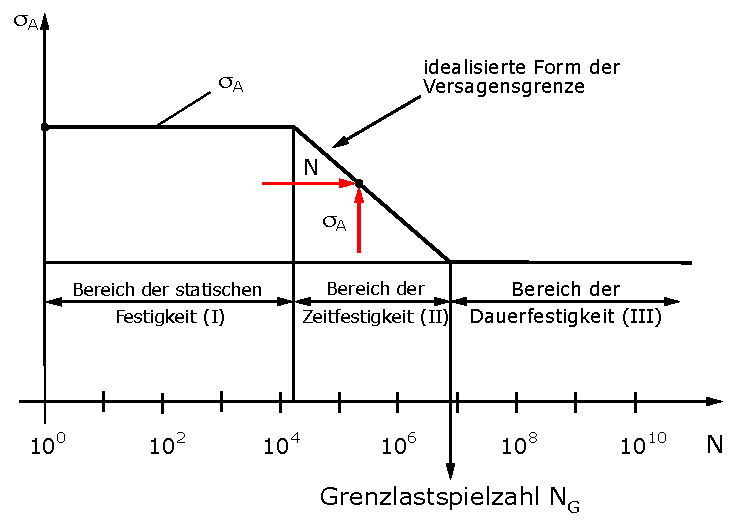
\includegraphics[width=\columnwidth]{graphics/woehler}
	
	Grenzlastspielzahl $N_G$: \\
	\begin{tabular}{lr@{$\:\approx\:$}l}
		harter Stahl & $N_G$ & $3 \cdot 10^6$ \\
		weicher Stahl & $N_G$ & $5 \cdot 10^6$ \\
		Cu, Cu-Legierung & $N_G$ & $50 \cdot 10^6$ \\
		harter Stahl & $N_G$ & $30\dots 100 \cdot 10^6$ -- $\infty$ \\
	\end{tabular}
% section: Wöhlerkurve (end)